\documentclass[10pt,letterpaper]{article}
\usepackage[utf8]{inputenc}
\usepackage[T1]{fontenc}
\usepackage[provide=*,spanish]{babel}
\usepackage{lmodern,geometry,amsmath,graphicx,xcolor,microtype,multicol,caption,fancyhdr,booktabs,listings,hyperref}
\usepackage{titlesec}
\geometry{top=1.8cm,bottom=2cm,left=1.75cm,right=1.75cm,headheight=14pt}
\setlength{\columnsep}{0.65cm}
\setlength{\parindent}{0pt}
\setlength{\parskip}{0.25em}
\titlespacing*{\section}{0pt}{1.6ex plus 0.3ex}{0.8ex}
\titlespacing*{\subsection}{0pt}{1.4ex plus 0.3ex}{0.7ex}
\widowpenalty=10000
\clubpenalty=10000
\definecolor{udecazul}{HTML}{003A70}
\definecolor{udecoro}{HTML}{C79A2B}
\hypersetup{colorlinks=true,linkcolor=udecazul,urlcolor=udecazul,pdftitle={Determinación de la aceleración de gravedad con un carrito},pdfauthor={Julio Bastías}}
\captionsetup{font=small,labelfont=bf,justification=centering,skip=4pt,hypcap=false}
\addto\captionsspanish{\renewcommand{\tablename}{Tabla}}

% Datos de la cabecera: completar antes de entregar.
\newcommand{\asignatura}{Asignatura [completar]}
\newcommand{\autores}{Julio Bastías}
\newcommand{\docente}{[completar]}
\newcommand{\ayudante}{[completar]}
\newcommand{\seccion}{Sección [completar]}
\newcommand{\fechaexperiencia}{Fecha [completar]}
\pagestyle{fancy}
\fancyhf{}
\lhead{\small Gravedad en un plano inclinado}
\rhead{\small \asignatura}
\cfoot{\small \thepage}
\renewcommand{\headrulewidth}{0.4pt}
\lstset{language=Python,basicstyle=\ttfamily\scriptsize,breaklines=true,columns=fullflexible,keepspaces=true,showstringspaces=false,numbers=left,numberstyle=\tiny\color{gray},numbersep=7pt,xleftmargin=12pt,frame=single,rulecolor=\color{gray!40}}

\begin{document}
\thispagestyle{empty}
\begin{center}
\begin{minipage}{0.46\textwidth}\raggedright
\includegraphics[width=0.68\linewidth]{figuras/logo_udec.png}\end{minipage}
\begin{minipage}{0.46\textwidth}\raggedleft
\includegraphics[width=0.68\linewidth]{figuras/logo_fcfm.png}\end{minipage}
{\color{udecoro}\rule{0.82\textwidth}{1.2pt}\par}
\vspace{0.15cm}
{\LARGE\bfseries\color{udecazul} Determinación de la aceleración de gravedad\par}
{\large Carrito sobre un plano inclinado\par}
\vspace{0.15cm}
{\small \autores\quad$\vert$\quad Universidad de Concepción, Chile\par}
{\small \asignatura\quad$\vert$\quad \seccion\quad$\vert$\quad \fechaexperiencia\par}
{\small Docente: \docente\qquad Ayudante: \ayudante\par}
\end{center}

\begin{abstract}
Se estimó la aceleración de gravedad mediante el descenso de un carrito desde reposo sobre un riel inclinado. A partir de siete puntos experimentales se calcularon las aceleraciones y se ajustó el modelo ideal $a=g\sin\theta$ con intercepto cero. Se obtuvo $g\approx9{,}97\,\mathrm{m/s^2}$, con una diferencia nominal de 1,6\,\% respecto de $9{,}81\,\mathrm{m/s^2}$. Se propagaron las incertidumbres de las posiciones, el ángulo y el tiempo para cada aceleración y estimación individual de gravedad. La incertidumbre temporal de 0,30 s es una estimación personal del cronometraje manual. No se determinó una incertidumbre de la pendiente ajustada.
\end{abstract}
\noindent\textbf{Palabras clave:} gravedad, plano inclinado, aceleración, incertidumbre.

\begin{multicols}{2}
\raggedcolumns
\section{Introducción}
El plano inclinado permite estudiar un movimiento más lento que la caída vertical. Al aumentar la inclinación, aumenta la componente del peso que impulsa el descenso. Se buscó determinar la gravedad relacionando el ángulo con la aceleración del carrito y estimar las incertidumbres experimentales.

\section{Teoría}
Para un carrito que parte desde reposo y se mueve con aceleración constante, $d=at^2/2$. Por tanto,
\begin{equation}
d=x_f-x_0,\qquad a=\frac{2d}{t^2}.
\end{equation}
Aquí $d$ es la distancia entre las posiciones final e inicial, y $t$ el tiempo usado. En el modelo ideal se desprecia el rozamiento, de modo que la componente del peso paralela al riel produce
\begin{equation}
a=g\sin\theta.
\end{equation}
Por tanto, al representar $a$ frente a $\sin\theta$ se obtiene una recta cuya pendiente es $g$ y cuyo intercepto es cero. Para cada medición también se puede estimar
\begin{equation}
g_i=\frac{2d_i}{t_i^2\sin\theta_i}.
\end{equation}

\section{Procedimiento experimental}
Se utilizó un riel con escala, un carrito, un indicador de inclinación y un cronómetro manual. Se soltó el carrito sin impulso y se registró el tiempo necesario para recorrer distancias de 49,5 o 69,5 cm, para las inclinaciones indicadas en la Tabla 1.

Se analizaron siete puntos, separando los dos de $5^\circ$ por tener distintos recorridos. La referencia inicial se midió una sola vez. Los tiempos utilizados corresponden principalmente a promedios de mediciones repetidas.

\begin{center}
\begin{minipage}{\linewidth}
\centering
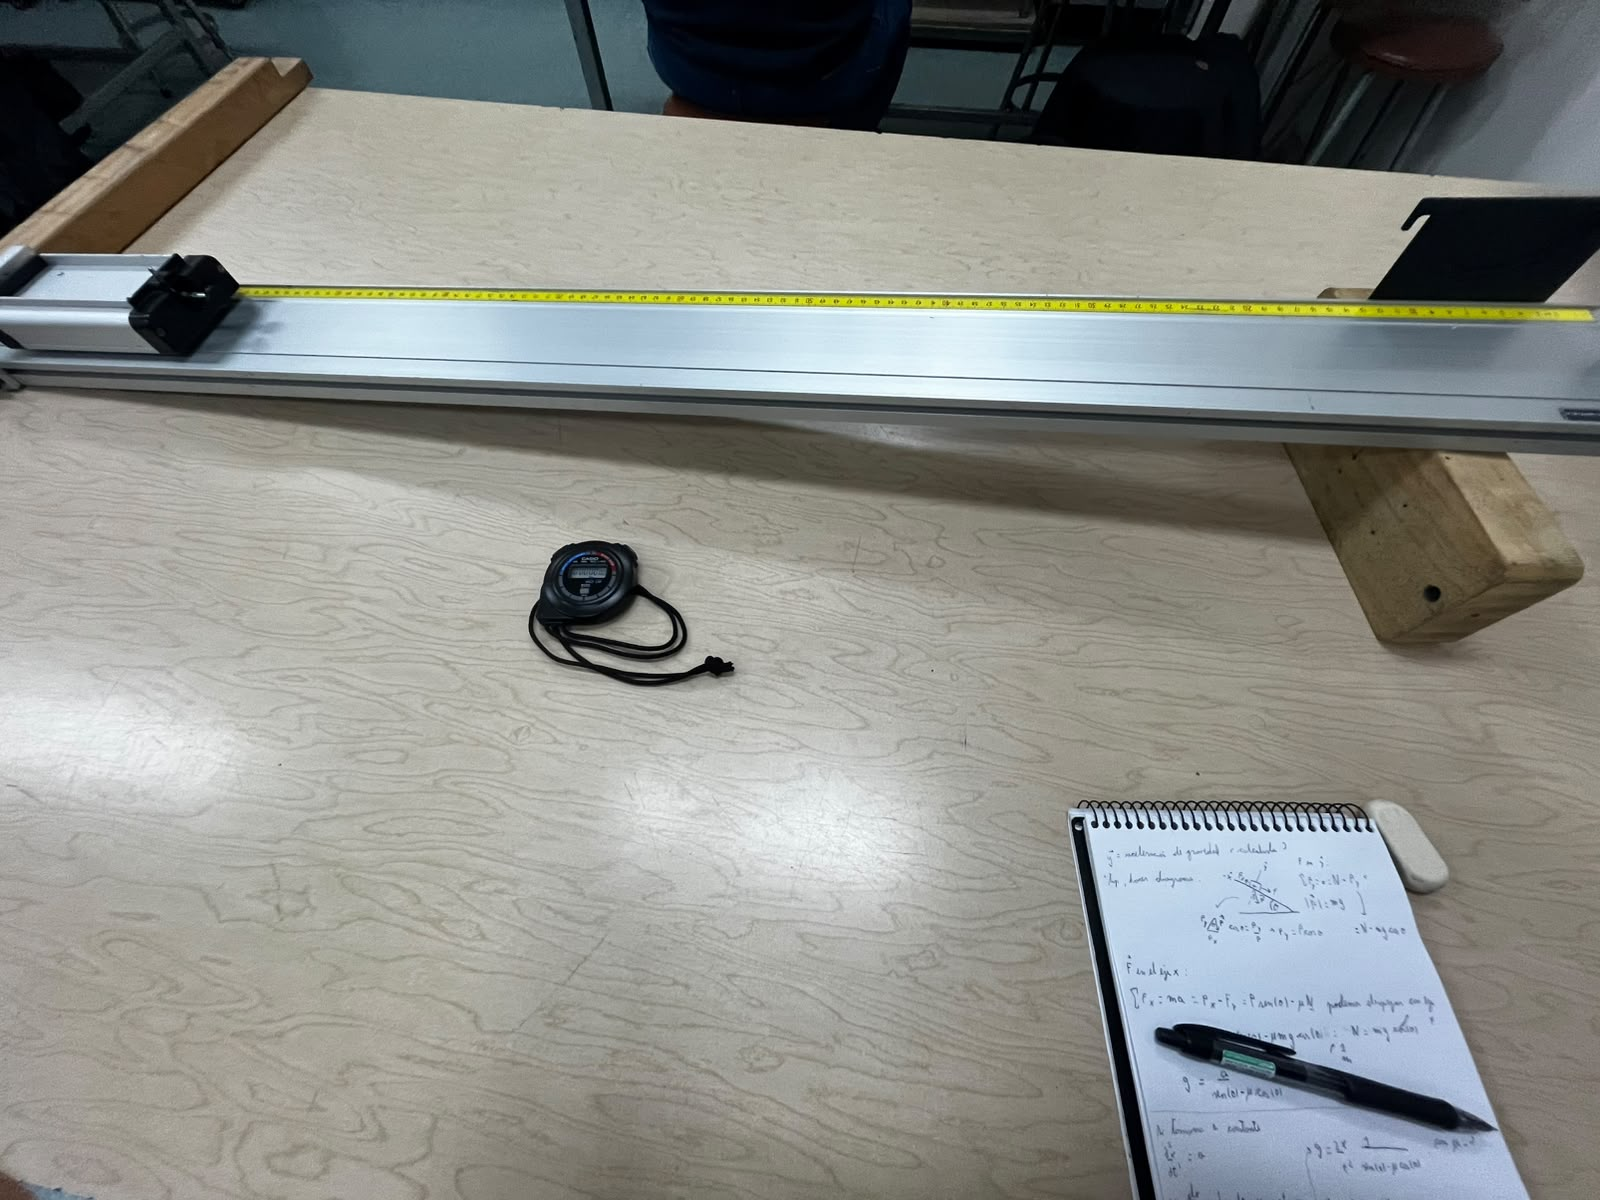
\includegraphics[width=0.75\linewidth]{montaje_carrito.jpg}
\captionof{figure}{Montaje del riel y carrito utilizado en la experiencia.}
\end{minipage}
\end{center}

\section{Resultados}
La Tabla 1 conserva los valores utilizados. Siguiendo el criterio de mitad de la división mínima [2], se adoptó $u_{x_0}=0{,}05$ cm para la regla de 1 mm y $u_\theta=0{,}5^\circ$ para el indicador de $1^\circ$. Se mantuvo $u_{x_f}=0{,}1$ cm porque el tope se desplazaba ligeramente y debía recolocarse entre medidas.

Se asignó provisionalmente $u_t=0{,}30$ s a cada tiempo utilizado. Es una estimación personal, no una desviación estándar ni un error estadístico del promedio; no se obtuvo mediante calibración ni se dividió por $\sqrt{N}$.

\begin{center}\begin{minipage}{\linewidth}\centering
\captionof{table}{Ángulo, distancia recorrida y tiempo de descenso.}
\small
\begin{tabular}{ccc}\toprule
$\theta$ ($^\circ$) & $d$ (m) & $t$ (s) \\ \midrule
1 & 0,695 & 3,185 \\
2 & 0,695 & 2,450 \\
3 & 0,695 & 1,855 \\
4 & 0,695 & 1,495 \\
5 & 0,495 & 1,125 \\
5 & 0,695 & 1,358 \\
10 & 0,695 & 0,850 \\
\bottomrule\end{tabular}
\end{minipage}\end{center}

\subsection{Propagación de errores}
Para las variables medidas independientes $q_j$ se aplicó la fórmula general de primer orden [3]:
\begin{equation}
u_f^2=\sum_j\left(\frac{\partial f}{\partial q_j}u_{q_j}\right)^2.
\end{equation}
Como $\partial d/\partial x_f=1$ y $\partial d/\partial x_0=-1$, tratando ambas lecturas como independientes,
\begin{equation}
u_d=\sqrt{u_{x_f}^2+u_{x_0}^2}\approx0{,}112\,\mathrm{cm}.
\end{equation}
Este valor intermedio se conserva sin redondear durante el cálculo. De $\partial a/\partial d=2/t^2$ y $\partial a/\partial t=-4d/t^3$ se obtiene
\begin{equation}
u_a=a\sqrt{\left(\frac{u_d}{d}\right)^2+
\left(\frac{2u_t}{t}\right)^2}.
\end{equation}
Para $g_i=a_i/\sin\theta_i$, las derivadas son $1/\sin\theta_i$ respecto de $a_i$ y $-g_i\cot\theta_i$ respecto de $\theta_i$. Así,
\begin{equation}
u_{g_i}=g_i\sqrt{\left(\frac{u_a}{a}\right)^2+
\left(\frac{u_\theta}{\tan\theta}\right)^2}.
\end{equation}
Se expresa $u_\theta$ en radianes. La Tabla 2 muestra los resultados con una cifra significativa en cada incertidumbre y el valor al mismo orden decimal [2].

\begin{center}\begin{minipage}{\linewidth}\centering
\captionof{table}{Magnitudes calculadas e incertidumbres.}
\small
\begin{tabular}{ccccc}\toprule
$\theta$ ($^\circ$) & $a$ & $u_a$ & $g_i$ & $u_{g_i}$ \\ \midrule
1 & 0,14 & 0,03 & 8 & 4 \\
2 & 0,23 & 0,06 & 7 & 2 \\
3 & 0,4 & 0,1 & 8 & 3 \\
4 & 0,6 & 0,2 & 9 & 4 \\
5 & 0,8 & 0,4 & 9 & 5 \\
5 & 0,8 & 0,3 & 9 & 4 \\
10 & 2 & 1 & 11 & 8 \\
\bottomrule\end{tabular}
\par\vspace{2pt}\footnotesize $a$, $u_a$, $g_i$ y $u_{g_i}$ en $\mathrm{m/s^2}$.
\end{minipage}\end{center}

\subsection{Ajuste de la gráfica}
Se ajustó $a$ frente a $\sin\theta$ por mínimos cuadrados ordinarios con intercepto cero, usando los siete puntos con igual peso. La pendiente fue
\begin{equation}
g\approx9{,}97\,\mathrm{m/s^2}.
\end{equation}
No se calculó una incertidumbre de esta pendiente. Las incertidumbres de la Tabla 2 corresponden a cada $a_i$ y $g_i$, no al ajuste. La diferencia nominal respecto de $9{,}81\,\mathrm{m/s^2}$ es 1,6\,\%.

\begin{center}\begin{minipage}{\linewidth}\centering
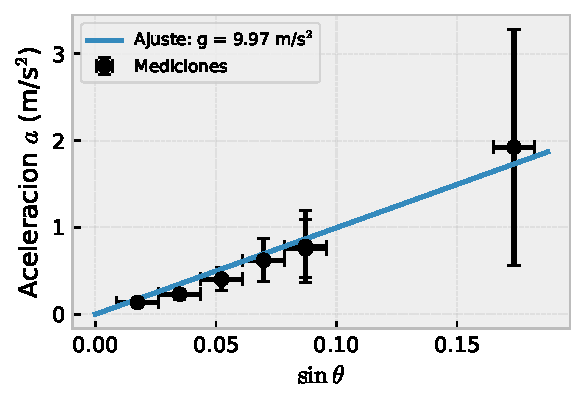
\includegraphics[width=\linewidth]{ajuste_gravedad.pdf}
\captionof{figure}{Aceleración frente a $\sin\theta$ y ajuste ideal. Las barras son $u_X=|\cos\theta|u_\theta$ y $u_a$, con $u_\theta=0{,}5^\circ$ y $u_t=0{,}30$ s estimada. Se grafican los valores sin redondear [1].}
\end{minipage}\end{center}

\section{Discusión de errores}
La aceleración aumenta en general con la inclinación, como predice el modelo ideal. Los dos puntos a $5^\circ$ dan aceleraciones próximas. La reacción al cronometrar, las lecturas y el reajuste del tope pueden producir variaciones aleatorias. Un desfase persistente del reloj o un cero angular mal ajustado producirían un error sistemático [2].

El tiempo interviene al cuadrado y la estimación $u_t=0{,}30$ s predomina en las barras verticales. Debe revisarse si se caracteriza mejor el cronometraje. En los ángulos pequeños y descensos breves los errores relativos son importantes, lo que limita la aproximación de primer orden. Las barras no representan intervalos de confianza. Además, la incertidumbre de la posición inicial es común a los recorridos y no disminuye por tener varios puntos.

Para mejorar la precisión se pueden usar fotopuertas, comprobar el ángulo con un instrumento más preciso y definir claramente las posiciones de salida y llegada. La cercanía del ajuste a la referencia no demuestra por sí sola una alta precisión experimental.

\section{Conclusiones}
El ajuste ideal con intercepto cero entregó $g\approx9{,}97\,\mathrm{m/s^2}$ y una diferencia nominal de 1,6\,\% respecto de la referencia. Se calcularon las incertidumbres de las aceleraciones y de las estimaciones individuales de gravedad mediante derivadas parciales. No se estimó una incertidumbre de la pendiente. El cronometraje manual y la incertidumbre angular limitan la precisión experimental.

\section*{Referencias}
[1] Laboratorio I. \textit{Clase 1: Gráficos}. Material del curso.

[2] Laboratorio I. \textit{Clase 2: Errores}. Material del curso.

[3] Laboratorio I. \textit{Clase 3: Medidas estadísticas}. Material del curso.
\end{multicols}

\clearpage
\appendix
\section{Código en Python}
El programa \nolinkurl{analisis_gravedad.py} lee únicamente \nolinkurl{datos_gravedad.txt}, imprime los resultados y genera \nolinkurl{ajuste_gravedad.pdf}. Se ejecuta con \texttt{python analisis\_gravedad.py} desde la carpeta del proyecto. Sigue seis bloques secuenciales y utiliza únicamente NumPy y Matplotlib. La pendiente se obtiene con $g=\sum_i X_i a_i/\sum_i X_i^2$, donde $X_i=\sin\theta_i$. Se conservan los valores originales del archivo; la incertidumbre angular se calcula con la división confirmada del indicador, en lugar del $1^\circ$ provisional que permanece en el archivo. La consola conserva cifras de control para revisar los cálculos.
\lstinputlisting{analisis_gravedad.py}
\end{document}
